\PassOptionsToPackage{unicode=true}{hyperref} % options for packages loaded elsewhere
\PassOptionsToPackage{hyphens}{url}
%
\documentclass[]{article}
\usepackage{lmodern}
\usepackage{amssymb,amsmath}
\usepackage{ifxetex,ifluatex}
\usepackage{fixltx2e} % provides \textsubscript
\ifnum 0\ifxetex 1\fi\ifluatex 1\fi=0 % if pdftex
  \usepackage[T1]{fontenc}
  \usepackage[utf8]{inputenc}
  \usepackage{textcomp} % provides euro and other symbols
\else % if luatex or xelatex
  \usepackage{unicode-math}
  \defaultfontfeatures{Ligatures=TeX,Scale=MatchLowercase}
\fi
% use upquote if available, for straight quotes in verbatim environments
\IfFileExists{upquote.sty}{\usepackage{upquote}}{}
% use microtype if available
\IfFileExists{microtype.sty}{%
\usepackage[]{microtype}
\UseMicrotypeSet[protrusion]{basicmath} % disable protrusion for tt fonts
}{}
\IfFileExists{parskip.sty}{%
\usepackage{parskip}
}{% else
\setlength{\parindent}{0pt}
\setlength{\parskip}{6pt plus 2pt minus 1pt}
}
\usepackage{hyperref}
\hypersetup{
            pdftitle={Global Climate Change, Oregon Wildfires, and Portland Air Quality},
            pdfauthor={Claire LeBlanc},
            pdfborder={0 0 0},
            breaklinks=true}
\urlstyle{same}  % don't use monospace font for urls
\usepackage[margin=1in]{geometry}
\usepackage{graphicx,grffile}
\makeatletter
\def\maxwidth{\ifdim\Gin@nat@width>\linewidth\linewidth\else\Gin@nat@width\fi}
\def\maxheight{\ifdim\Gin@nat@height>\textheight\textheight\else\Gin@nat@height\fi}
\makeatother
% Scale images if necessary, so that they will not overflow the page
% margins by default, and it is still possible to overwrite the defaults
% using explicit options in \includegraphics[width, height, ...]{}
\setkeys{Gin}{width=\maxwidth,height=\maxheight,keepaspectratio}
\setlength{\emergencystretch}{3em}  % prevent overfull lines
\providecommand{\tightlist}{%
  \setlength{\itemsep}{0pt}\setlength{\parskip}{0pt}}
\setcounter{secnumdepth}{0}
% Redefines (sub)paragraphs to behave more like sections
\ifx\paragraph\undefined\else
\let\oldparagraph\paragraph
\renewcommand{\paragraph}[1]{\oldparagraph{#1}\mbox{}}
\fi
\ifx\subparagraph\undefined\else
\let\oldsubparagraph\subparagraph
\renewcommand{\subparagraph}[1]{\oldsubparagraph{#1}\mbox{}}
\fi

% set default figure placement to htbp
\makeatletter
\def\fps@figure{htbp}
\makeatother


\title{Global Climate Change, Oregon Wildfires, and Portland Air Quality}
\author{Claire LeBlanc}
\date{}

\begin{document}
\maketitle

\hypertarget{oregon-wildfires-and-air-quality}{%
\subsection{Oregon Wildfires and Air
Quality}\label{oregon-wildfires-and-air-quality}}

On September 9th and 10th, a windstorm roared through the Pacific
Northwest. After an extremely dry summer, this created a ``once in a
generation'' wildfire event in Oregon, with over one million acres
burning and multiple lives being lost. In Portland, we avoided the worst
of the consequences. We were not forced to evacuate, and we did not lose
our homes and neighborhoods to the flames.

One of the main effects for Portlanders was air quality in the
``Hazardous'' range for over a week, sometimes rising to levels above
the EPA scale. While this had impacts on everyone in Portland, the
impacts were not felt equally. For those experiencing homelessness,
those with essential jobs, and those without an air sealed home or the
resources to buy an air filter, the effects were much more severe.

\begin{figure}
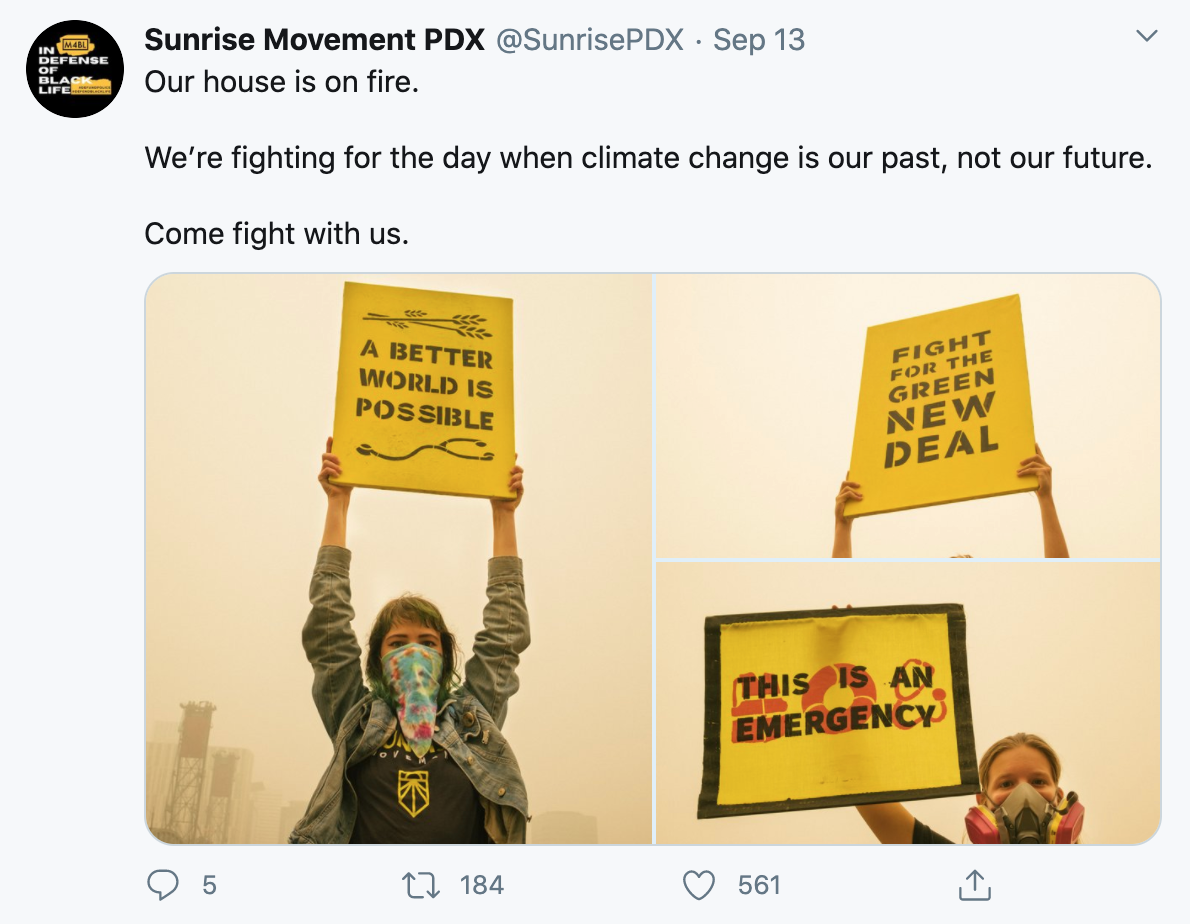
\includegraphics[width=0.5\linewidth]{Screen Shot 2020-09-21 at 8.55.15 PM} 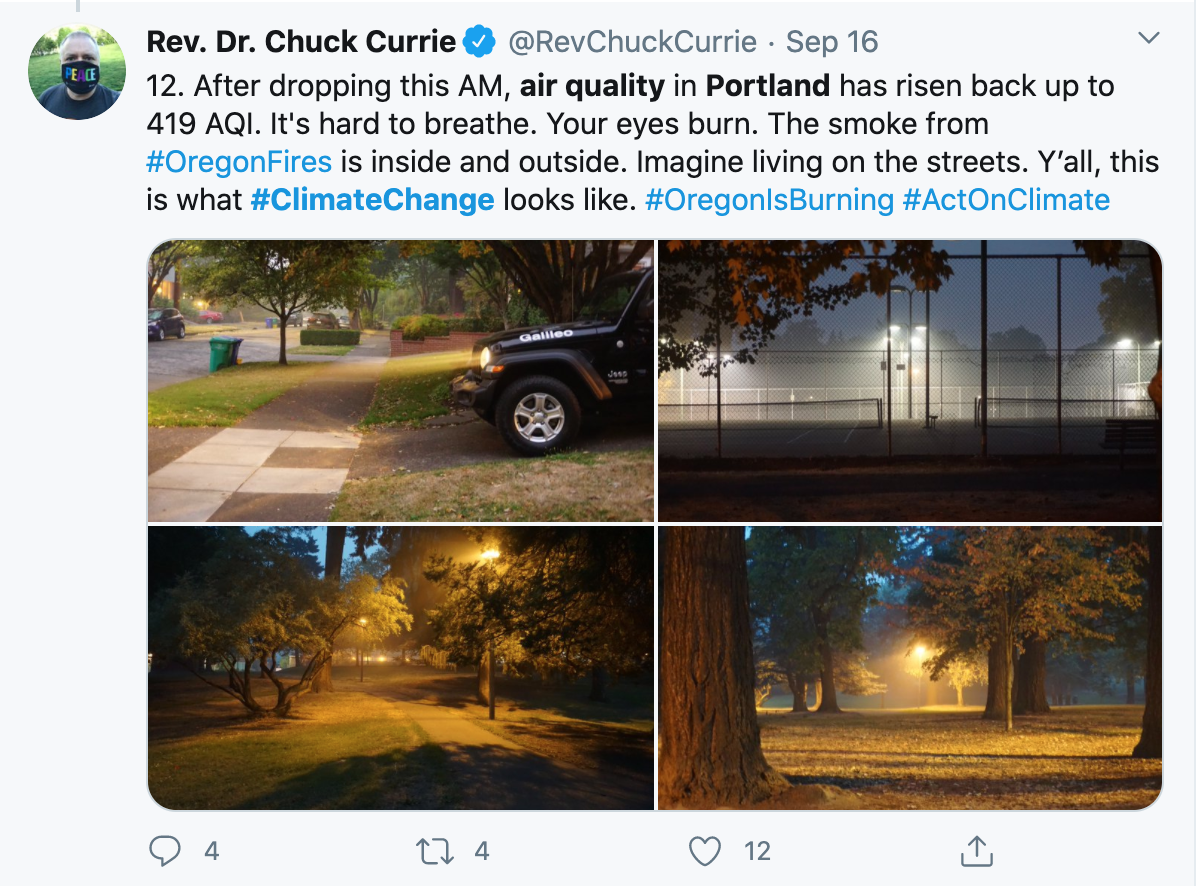
\includegraphics[width=0.5\linewidth]{Screen Shot 2020-09-21 at 9.03.22 PM} \caption{Figure 1: Twitter posts connecting the smoke in Portland, OR to climate change}\label{fig:unnamed-chunk-1}
\end{figure}

Many in Portland connected the hazardous air quality to climate change
(Figure 2). Climate change increases the area burned by wildfires,
therefore also increasing smoke (7). According the Oregon Department of
Forestry, the number or acres burned by wildfires has been increasing in
recent years (figure 2).

\begin{figure}
\centering
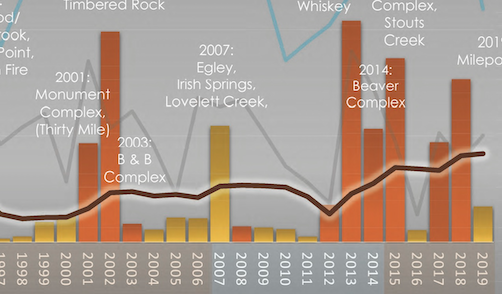
\includegraphics{Screen Shot 2020-09-26 at 12.53.31 PM.png}
\caption{Figure 2: Graph by the Oregon Forestry Department. The Orange
and Yellow bars show the area burned that year. The black line shows the
increasing trend of acres burned over time. The grah has been zoomed in
on the portion from 1999 to 2019 because that is where I will be
focusing my analysis.}
\end{figure}

But is climate change causing a perceptible change in Portland's air
quality?

Liu et al.~investigated this question using a chemical transport model.
With this model, they looked at the wildfire smoke risk of different
counties in the Western United States in 2009 and in 2051 to see how
climate change might increase or decrease this risk. They found that
Clackamas, Washington and Multnomah counties all had a risk of 4 (with 5
being the highest) in 2009. By 2051, their model showed Clackamas and
Washington increased to the highest risk level, while Multnomah remained
at the level 4 risk. (4)

Using Portland temperature and air quality data, I investigated these
predictions by seeing how air quality is changing in Portland, and
whether these can be connected to our changing climate.

\hypertarget{portland-is-getting-hotter}{%
\subsection{Portland is Getting
Hotter}\label{portland-is-getting-hotter}}

Daily temperature data collected at the Portland International Airport
was obtained from the NOAA database. From this data, monthly means were
calculated and graphed. I hypothesized that there would be an increase
in daily maximum temperature over the four months looked at: June, July,
August, and September. To test this, I looked at whether the null
hypothesis, that there is no increase in temperature, could be rejected
using a 95\% confidence interval.

\begin{figure}
\includegraphics[width=0.5\linewidth]{Region_87336_files/figure-latex/temp graphs-1} \includegraphics[width=0.5\linewidth]{Region_87336_files/figure-latex/temp graphs-2} \includegraphics[width=0.5\linewidth]{Region_87336_files/figure-latex/temp graphs-3} \includegraphics[width=0.5\linewidth]{Region_87336_files/figure-latex/temp graphs-4} \caption{Figure 3: Graphs of average daily max temperature in June, July, August, and September. All four months showed a significant trend. For June, p = 0.03627 < 0.05 and Adjusted R-squared = 0.04132. For July, For July, p = 0.0223 < 0.05 and the Adjusted R-squared = 0.0512. For August, p = 8.038 x 10^-6 < 0.05 and the Adjusted R-squared = 0.2096. For September, p = 0.03693 < 0.05 and Adjusted R-squared = 0.04095.}\label{fig:temp graphs}
\end{figure}

As you can see from Figure 3, all four months show an increase in
temperature. Additionally, for all four months, the null hypothesis is
rejected and the increase in temperature is found to be significant.

Notably, in August, one of the main fire season months, this trend is
particularly strong, with an extremely small p-value (p = 8.038 x
10\^{}-6). August also had an adjusted R-squared value of about .2,
meaning that 20\% of the variation in the data can be explained by
simply looking at the year. This is very high for climate data which, as
shown in Figure 1, tends to vary greatly by year, suggesting that
climate change is having a large effect in August in particular. In
addition, the August trendline had the largest slop, with temperature
increasing by 0.037 degrees per year. While this may seem small, it
corresponds to a two degree increase over fifty years, which will have a
significant effect on a variety of climatic and ecological systems.

It is important to note, however, that this data is for Portland only,
not for all of Oregon. Temperature changes may be slightly different in
other parts of the state, where wildfires occur. This data does show,
however, that regardless of smoke, climate change in influencing
Portland by increasing temperatures.

\hypertarget{air-quality-is-not-getting-worse-but-its-not-getting-better}{%
\subsection{Air Quality is Not Getting Worse (But it's Not Getting
Better)}\label{air-quality-is-not-getting-worse-but-its-not-getting-better}}

I obtained air quality data from the EPA, which compiled daily air
quality measurements for a variety of pollutants from a variety of
different locations around Portland.

The EPA monitors and measures air quality under the Clean Air Act of
1970. It then ranks each pollutant on a scale known as the Air Quality
Index (AQI) which ranges from 0-500, where higher values represent
greater pollution and health risk. The EPA uses the AQI to measure the
concentrations of five main pollutants: particulate matter, ground-level
ozone, carbon monoxide, sulfur dioxide, and nitrogen dioxide. (1)

Smoke from fires contains many different chemicals, but this analysis
will focus on one of the most dangerous components, PM 2.5, or
particulate matter with a diameter of 2.5 micrometers and smaller. These
particles are particularly dangerous because, due to their small size,
they can travel deep in the lungs (1). Focusing on PM 2.5, however, also
limited the length of this analysis, as PM 2.5 data was only available
starting in 1999.

The data from the EPA provided a daily PM 2.5 value, which I used to
create and graph monthly averages.

Like with temperature, I hypothesized that air quality decreased over
time (causing increasing AQI values and a positive trend in the graph).
To test this, I tested the null hypothesis, that there was no increasing
or decreasing trend. A 95\% confidence interval was used for this
analysis as well.

\begin{figure}
\includegraphics[width=0.5\linewidth]{Region_87336_files/figure-latex/AQ graphs-1} \includegraphics[width=0.5\linewidth]{Region_87336_files/figure-latex/AQ graphs-2} \includegraphics[width=0.5\linewidth]{Region_87336_files/figure-latex/AQ graphs-3} \includegraphics[width=0.5\linewidth]{Region_87336_files/figure-latex/AQ graphs-4} \caption{Figure 4: Graphs of average daily PM 2.5 AQI value for June, July, August and September. For June, p = 0.01491 < 0.05, Adjusted R-squared = 0.2357, and slope = -1.539. For July p = 0.03258 < 0.05, Adjusted R-squared = 0.1775, and slope = -2.461. For August, p = 0.09299 > 0.05, Adjusted R-squared = 0.09619, and slope = 2.542. For September, p = 0.651 > 0.05, Adjusted R-squared = -0.04105, and slope = 0.5974. }\label{fig:AQ graphs}
\end{figure}

Figure 4 shows the average AQI PM 2.5 reading for Portland from 1999 to
2019. For the months of June and July, both my hypothesis and the null
hypothesis were rejected. Instead, both months showed a significant
decreasing trend in AQI. Additionally, both had very high Adjusted
R-squared values of 0.24 and 0.18 respectively, meaning that 24\% and
18\% of the variation in the data can be explained by time alone. This
suggests that, for June and July, there is a strong correlation between
time and decreasing AQI values (improving air quality).

In August and September, this trend was not maintained. Instead, both
graphs showed an increase in the average AQI value over time. This
increase, however, was not found to be significant within a 95\%
confidence interval. If we lower to a 90\% confidence interval, however,
the increasing trend in August is found to be significant (p = 0.09299
\textgreater{} 0.10).

This data seems to imply that forest fires and climate change are not
having a perceptible impact on air quality, but that may not be the full
story. According to the EPA/National Park Service Visibility Program
(known as IMPROVE), PM 2.5 AQI values have been improving throughout the
US due to EPA regulations after the Clean Air Act of 1970 (7). Many
other sources besides wildfire pollute PM 2.5, such as construction
sites, fields, smokestacks, and reactions between other pollutants in
the atmosphere (1). Regulations and decreases in these forms of
pollution have contributed to a general decrease in PM 2.5 AQI and an
improvement in air quality. Increases in forest fire smoke, however, may
be one reason that in August and September (biggest fire months), PM 2.5
AQI is not decreasing.

It is difficult to prove that this lack of improvement in PM 2.5
concentrations is due to forest fires. O'Dell et al.~investigated this
question. Looking at the Western United States, they combined PM 2.5
measurments with satellite smoke data to try and determine which days
and locations were ``smoke influenced.'' When excluding these smoke
days, there was a significant decrease in PM 2.5 values, suggesting that
increases in air pollution from wildfires is cancelling out decreases in
pollution from other sources. (7)

\hypertarget{consequences-of-increased-smoke}{%
\subsection{Consequences of Increased
Smoke}\label{consequences-of-increased-smoke}}

\begin{figure}
\centering
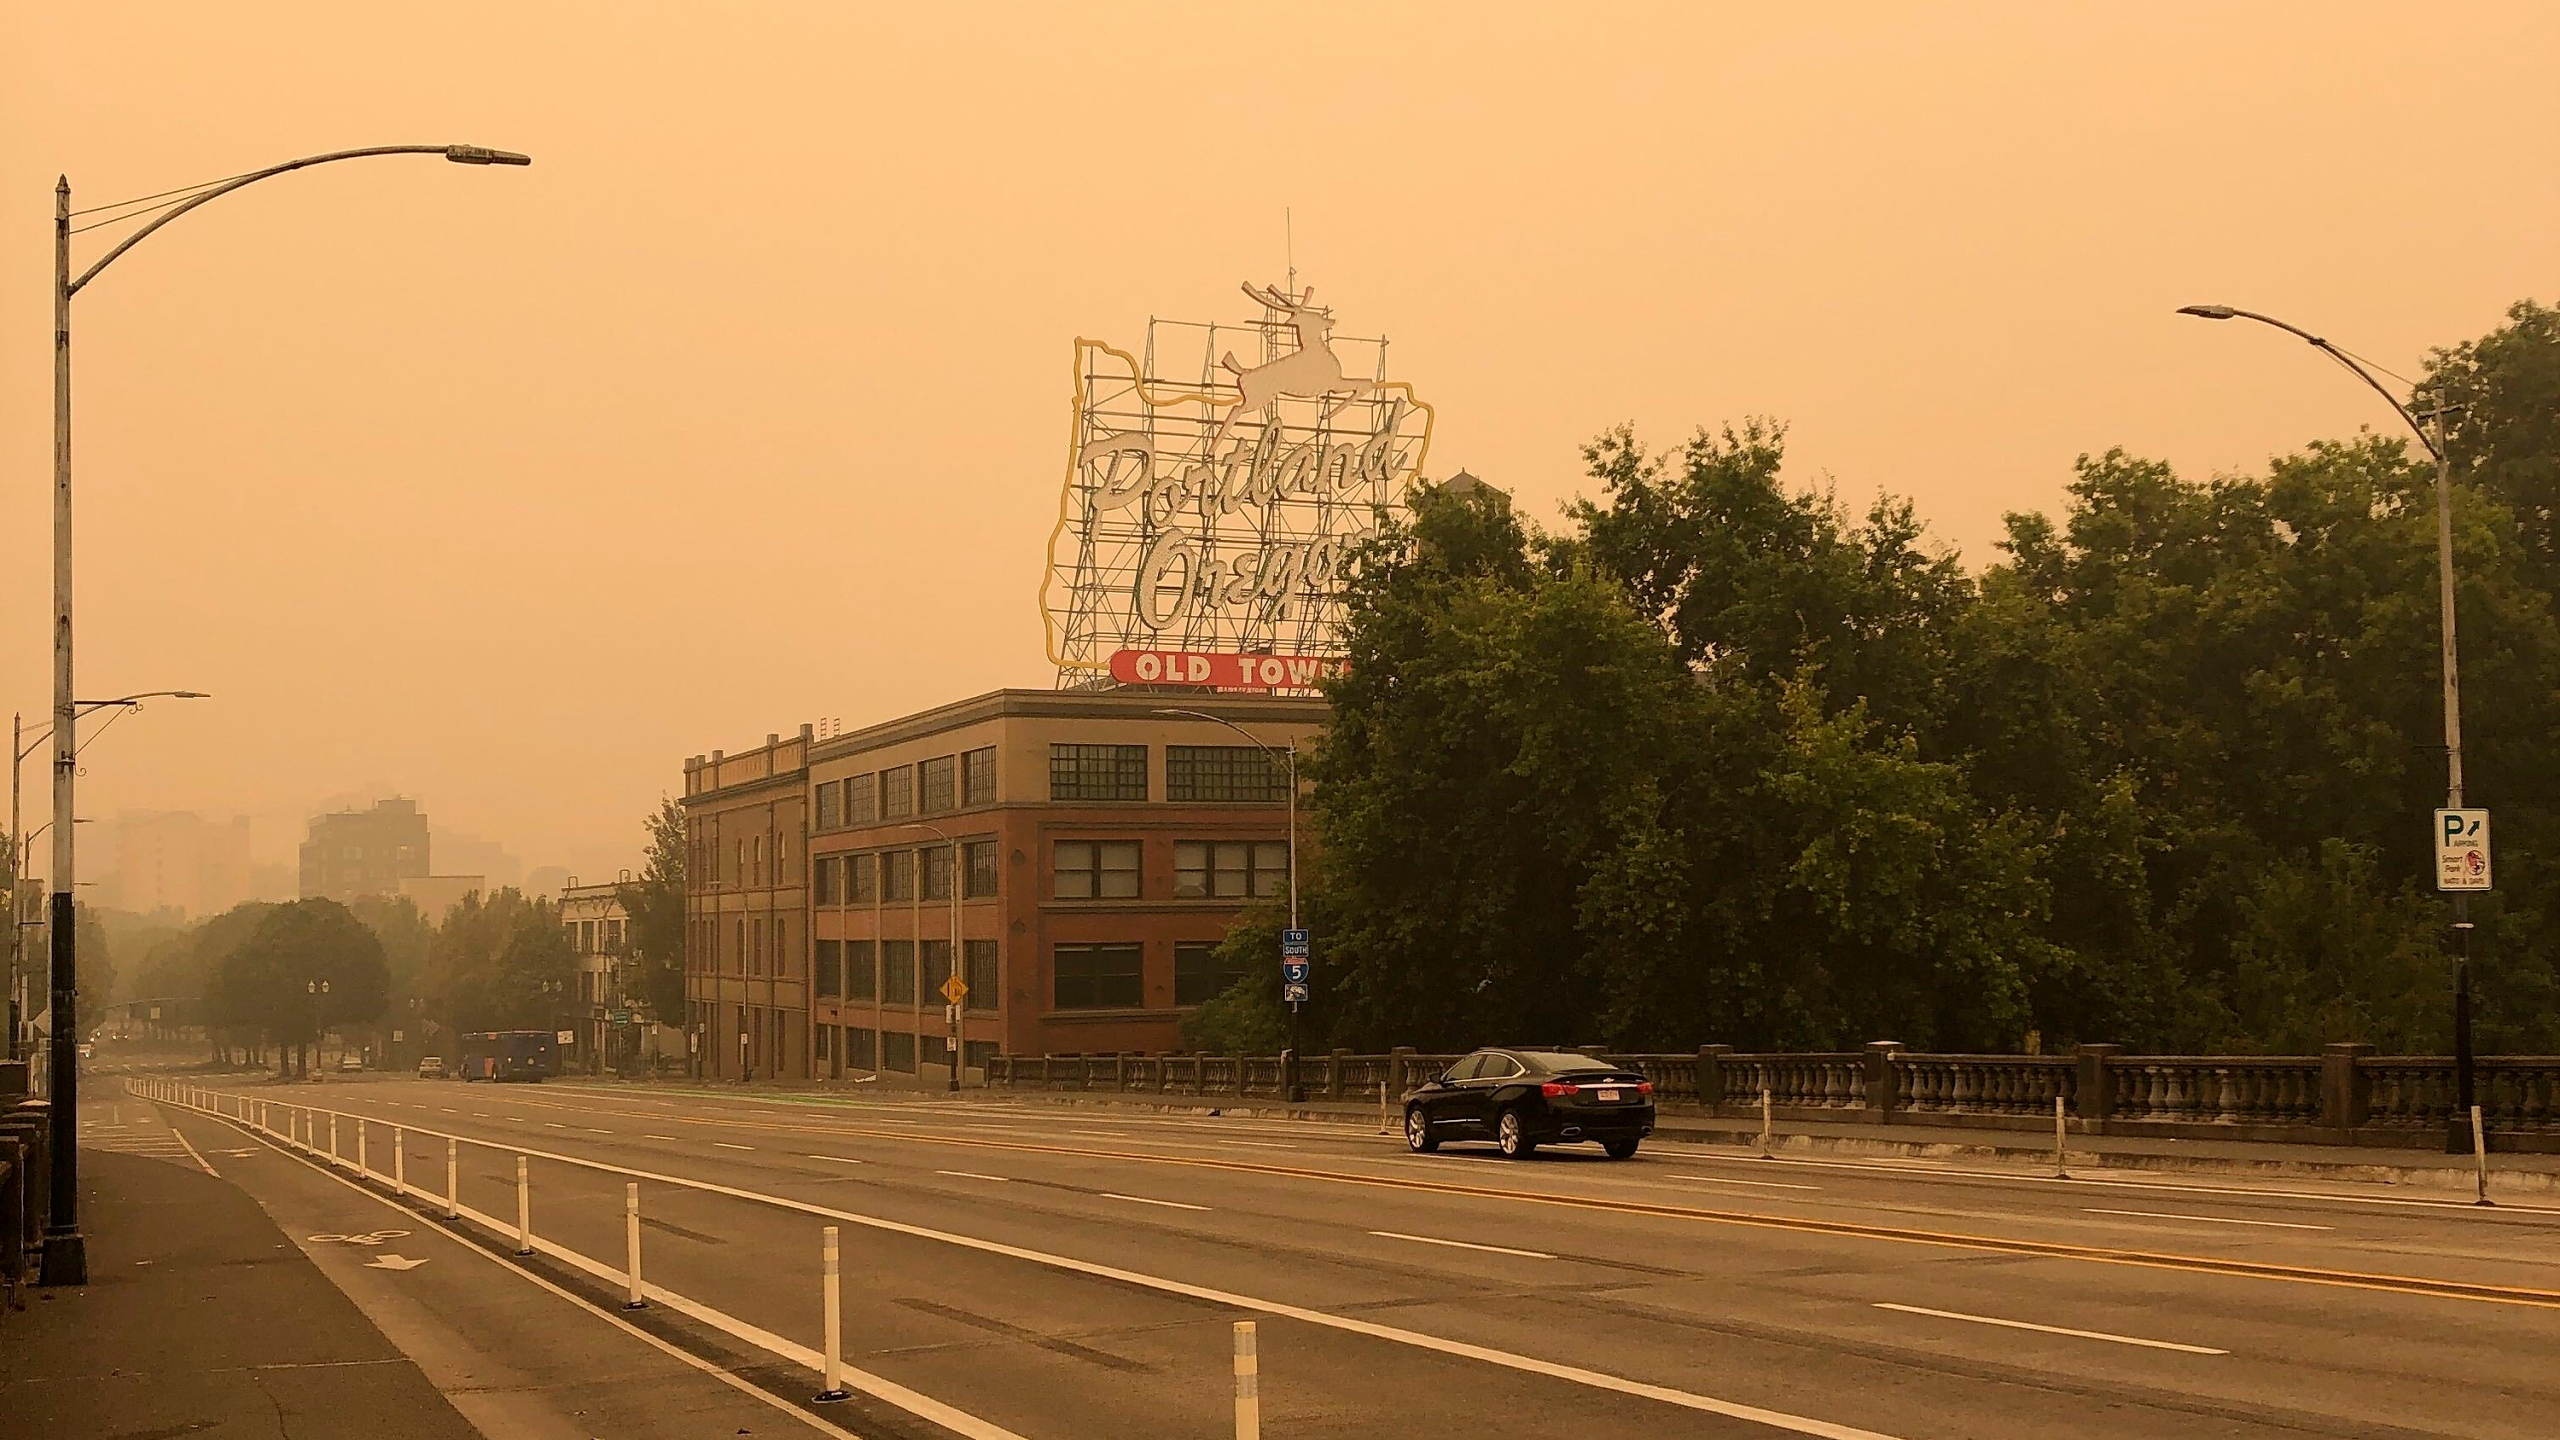
\includegraphics{AP20257021718485.jpg}
\caption{Smoke due to wildfires in Portland, OR on September 12, 2020.
Source:
\url{https://www.koin.com/news/wildfires/trash-collection-delayed-by-hazardous-air-quality-in-portland-metro/}}
\end{figure}

The connection between wildfire smoke and climate change provides a lot
of potential. When it was passed, the Clean Air Act received bipartisan
support, and the fight for clean air has consistently managed to bring
together a broad coalition of public health activists, social justice
activists, and climate activists (2). Connecting climate change to
decreased air quality could provide an opportunity to unite these
activists around climate change.

\hypertarget{public-health}{%
\subsubsection{Public Health}\label{public-health}}

A variety of studies have investigated the health impacts of exposure to
wildfire smoke. Lui et al.~reviewed 61 studies investigating the
relationship between wildfire smoke and health. They reported that 90\%
of the studies found a significant association between wildfire smoke
and an increased risk of respiratory morbidity (5). Another study by
Jones et al.~found that smoke-related health costs rose 1256\% in Oregon
from 2005 to 2015, and that wildfire smoke related health costs in the
Western US totaled \$165 million per year (3).

\hypertarget{social-justice}{%
\subsubsection{Social Justice}\label{social-justice}}

Poor air quality from wildfires is also a climate justice issue. For
example, people experiencing homelessness experience a greater exposure
to wildfire smoke. According to the US Interagency Council on
Homelessness, about 15,876 people experience homelessness on any given
day in Oregon and about 4,015 of those people are in Multnomah county
(8). After adjusting for population, Portland has one of the highest
rates of homelessness in the country, due to a lack of affordable
housing and mental health resources (8). Poor air quality will
undoubtedly affect these individuals more, as they often do not have a
safe indoor space where they can escape the poor air quality for long
periods of time.

Additionally, those in the essential workforce may be required to go
outside and work in the dangerous air quality. People with low incomes
may not have the resources to afford air filters or to air seal their
home to keep out the smoke.

Studies have also found that the health effects of poor air quality
disproportionately affect minority groups. These disparities are caused
by the systematic racism that pervades all levels of US society. One
study by Liu et al.~looking at individuals over 65 years of age found
that a higher fraction of Blacks were exposed to more than one smoke
wave. They also found that Blacks had a 21.7\% increased rate of
respiratory admissions to hospitals, compared to a 6.9\% increase for
whites. (6)

\hypertarget{what-can-we-do}{%
\subsection{What can we do?}\label{what-can-we-do}}

With an election coming up, you may be tired of the advice to vote, but
I am going to go give it anyway. Vote! Vote for candidates on the local,
regional, and national level that believe in climate change and will
make it a priority to solve this problem.

Beyond that, this issue provides the opportunity to unite a variety of
activists to fight for clean air by limiting carbon dioxide emissions,
just like in the 1960s and 70s. In social media posts about the fires
and climate change, focus also on the climate justice and health
implications of the smoke to highlight how this is an interdisciplinary
issue.

Lastly, lawyers and activists can use this issue to press the EPA to
regulate carbon dioxide emissions. While the Supreme Court has
previously given the EPA the right to regulate carbon dioxide emissions,
that right is not absolute and carbon dioxide is still not heavily
regulated. And as the court becomes more conservative and possibly less
reliant on precedent, the EPA may no longer have the right to regulate
carbon dioxide.

Connecting rising carbon dioxide levels to worsening levels of PM 2.5
could provide a solution. On the EPA's website, it states that its
``national and regional rules to reduce emissions of pollutants that
form PM'' will help reduce PM levels. The EPA is already regulating
other pollutants that cause an increase in particulate matter in order
to decrease particulate matter and they could and should do the same
with carbon dioxide.

\hypertarget{citations}{%
\subsubsection{Citations}\label{citations}}

\begin{enumerate}
\def\labelenumi{\arabic{enumi}.}
\tightlist
\item
  AQI Basics {[}Internet{]}. {[}place unknown{]}: AirNow; {[}date
  unknown; cited 2020 Sep 26{]}. Available from:
  \url{https://www.airnow.gov/aqi/aqi-basics/}
\item
  Allison JE, Press D, Horowitz C, Millard-Ball A, Pincetl S. Chapter 7.
  Paths to Carbon Neutrality: Lessons from California. Collabra Psychol
  {[}Internet{]}. 2016 {[}cited 2020 Sep 26{]};2(1):1-15. doi:
  10.1525/collabra.66
\item
  Jones BA, Berrens RP. Application of an Original Wildfire Smoke Health
  Cost Benefits Transfer Protocol to the Western US, 2005-2015. Environ
  Manage {[}Internet{]}. 2017 Sep {[}cited 2020 Sep 19{]};60:809-822.
  \url{doi:10.1007/s00267-017-0930-4}
\item
  Liu JC, Mickley LJ, Sulprizio MP, Dominici F, Yue X, Ebisu K, Anderson
  GB, Khan RFA, Bravo MA, Bell ML. Particulate Air Pollution from
  Wildfires in the Western US under Climate Change. Clim Change
  {[}Internet{]}. 2016 Oct {[}cited 2020 Sep 19{]};138(3):655-666. doi:
  10.1007/s10584-016-1762-6
\item
  Liu JC, Pereira G, Uhl SA, Bravo MA, Bell ML. A systematic review of
  the physical health impacts from non-occupational exposure to wildfire
  smoke. Environ Res {[}Internet{]}. 2015 Jan {[}cited 2020 Sep
  19{]};136:120-132. doi: 10.1016/j.envres.2014.10.015
\item
  Liu JC, Wilson A, Mickley LJ, Ebisu K, Sulprizio MP, Wang Y, Peng RD,
  Yue X, Dominici F, Bell ML. Who Among the Elderly Is Most Vulnerable
  to Exposure to and Health Risks of Fine Particulate Matter From
  Wildfire Smoke. AM J Epidemiol {[}Internet{]}. 2017 Sep {[}cited 2020
  Sep 26{]};186(6):730-735. doi: 10.1093/aje/kwx141
\item
  O'Dell K, Ford B, Fischer EV, Pierce JR. Contribution of Wildland-Fire
  Smoke to US PM2.5 and Its Influence on Recent Trends. Environ Sci
  Technol {[}Internet{]}. 2019 Jan {[}cited 2020 Sep
  19{]};53(4):1797-1804. doi: /10.1021/acs.est.8b05430
\item
  SOH: State and CoC Dashboards {[}Internet{]}. Washington, DC: National
  Alliance to End Homelessness; {[}updated 2019; cited 2020 Sep 26{]}.
  Available from:
  \url{https://endhomelessness.org/homelessness-in-america/homelessness-statistics/state-of-homelessness-dashboards/?State=Oregon}
\end{enumerate}

\end{document}
